% Created 2014-06-10 Tue 22:50
\NeedsTeXFormat{LaTeX2e}
\ProvidesClass{try}
\documentclass[final,paper=a4,paper=portraitmpagesize=auto,fontsize=11pt,ngerman]{scrartcl}
\usepackage[ngerman, germanb]{babel}
\usepackage[utf8]{inputenc}
\usepackage{fancyhdr}
\usepackage{amsmath}
\usepackage{amssymb}
\usepackage{lmodern}
\usepackage{graphicx}
\usepackage{geometry} %ist für die Größere der Seite da, wie groß darf der Textkörper sein.

% ~~~~~~~~~~~~~~~~~~~~~~~~~~~~~~~~~~~~~~~~~~~~~~~~~~~~~~~~~~~~~~~~~~~~~~~~
% fonts of headings
% ~~~~~~~~~~~~~~~~~~~~~~~~~~~~~~~~~~~~~~~~~~~~~~~~~~~~~~~~~~~~~~~~~~~~~~~~
\setkomafont{sectioning}{\normalfont\sffamily} % \rmfamily
\setkomafont{descriptionlabel}{\itshape}
\setkomafont{pageheadfoot}{\normalfont\normalcolor\small\sffamily}
\setkomafont{pagenumber}{\normalfont\sffamily}

\setkomafont{caption}{\footnotesize\normalfont}
\setkomafont{captionlabel}{\footnotesize\normalfont}

\date{\today}

% enlarge page
\geometry{tmargin=35mm,bmargin=30mm,lmargin=30mm,rmargin=30mm}

% skip between paragraphs
\setlength{\parskip}{1ex}
% ... and no indentation at start of a new paragraph
\setlength{\parindent}{0ex}

% mathe makros
\newcommand{\R}{\mathbb{R}}
\newcommand{\N}{\mathbb{N}}
\newcommand{\Z}{\mathbb{Z}}
\newcommand{\Q}{\mathbb{Q}}
\newcommand{\C}{\mathbb{C}}
\newcommand{\qed}{$ \hfill \Box $}
\newcommand{\im}[1]{\text{Im}\left(#1\right)}
\newcommand{\re}[1]{\text{Re}\left(#1\right)}

%physics
\usepackage[]{units}

% überschriften und son zeug
\pagestyle{fancy}
\lhead{Experimentalphysik 1 - M2} \chead{} \rhead{Maik Schünemann, Marcel Jacobse} 
\lfoot{} \cfoot{\thepage} \rfoot{} 
\renewcommand{\headrulewidth}{0.4pt} 
\usepackage[utf8]{inputenc}
\usepackage[T1]{fontenc}
\usepackage{fixltx2e}
\usepackage{graphicx}
\usepackage{longtable}
\usepackage{float}
\usepackage{wrapfig}
\usepackage{rotating}
\usepackage[normalem]{ulem}
\usepackage{amsmath}
\usepackage{textcomp}
\usepackage{marvosym}
\usepackage{wasysym}
\usepackage{amssymb}
\usepackage{hyperref}
\tolerance=1000
\author{Maik Schünemann}
\date{\today}
\title{Cognitive Systems Excercise 3}
\hypersetup{
 pdfkeywords={},
  pdfsubject={},
  pdfcreator={Emacs 24.3.1 (Org mode 8.2.6)}}
\begin{document}

\maketitle
\tableofcontents


\rule{\linewidth}{0.5pt}
\section{Excercise 1}
\label{sec-1}

\subsection{Concept of the extension}
\label{sec-1-1}
\subsubsection{Additional Components}
\label{sec-1-1-1}
We added group recognizer components to our cognitive
architecture, one for each group of proximity.
They extend the counting/recognizing visual routines - 
functionality of excercise 2. 
\subsubsection{Interplay between the components}
\label{sec-1-1-2}
To model human behaviour, we only concentrate on the filled
regions of the visual stimulus. We extended the peripheral view
component to quickly scan the picture to find the regions of 
the stimuli that are filled. 
On this regions we invoke the actual algorithm to count the 
groups (implemented in the components above).
If we have found a non-empty cell our system looks at all adjacent
cells if they also belong to the group. It does this until it has
found the whole group the cell belongs to.
It then continues looking for other groups but knows what cells it
has looked at before and doesn't revisit them.
The components for recognizing groups of proximity, color, shape 
only behave differently when they decide whether the adjacent cell
belongs to the same group or not

\subsubsection{Examples: \\}
\label{sec-1-1-3}

\begin{figure}[hbtp]
    \centering
    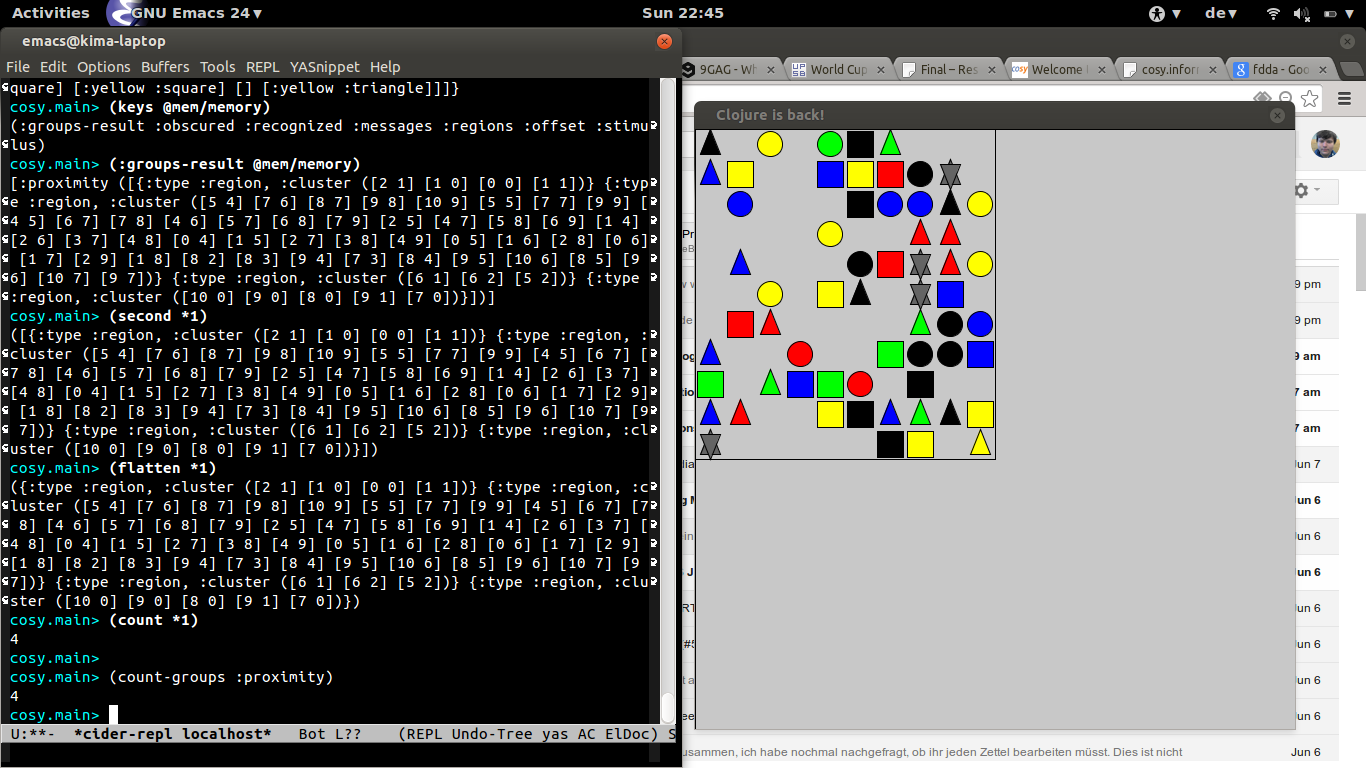
\includegraphics[width= 0.7 \textwidth]{grouping_example}
    \caption{Recognizing 4 groups of proximity}
    \label{fig:aufbau}
\end{figure}

\begin{figure}[hbtp]
    \centering
    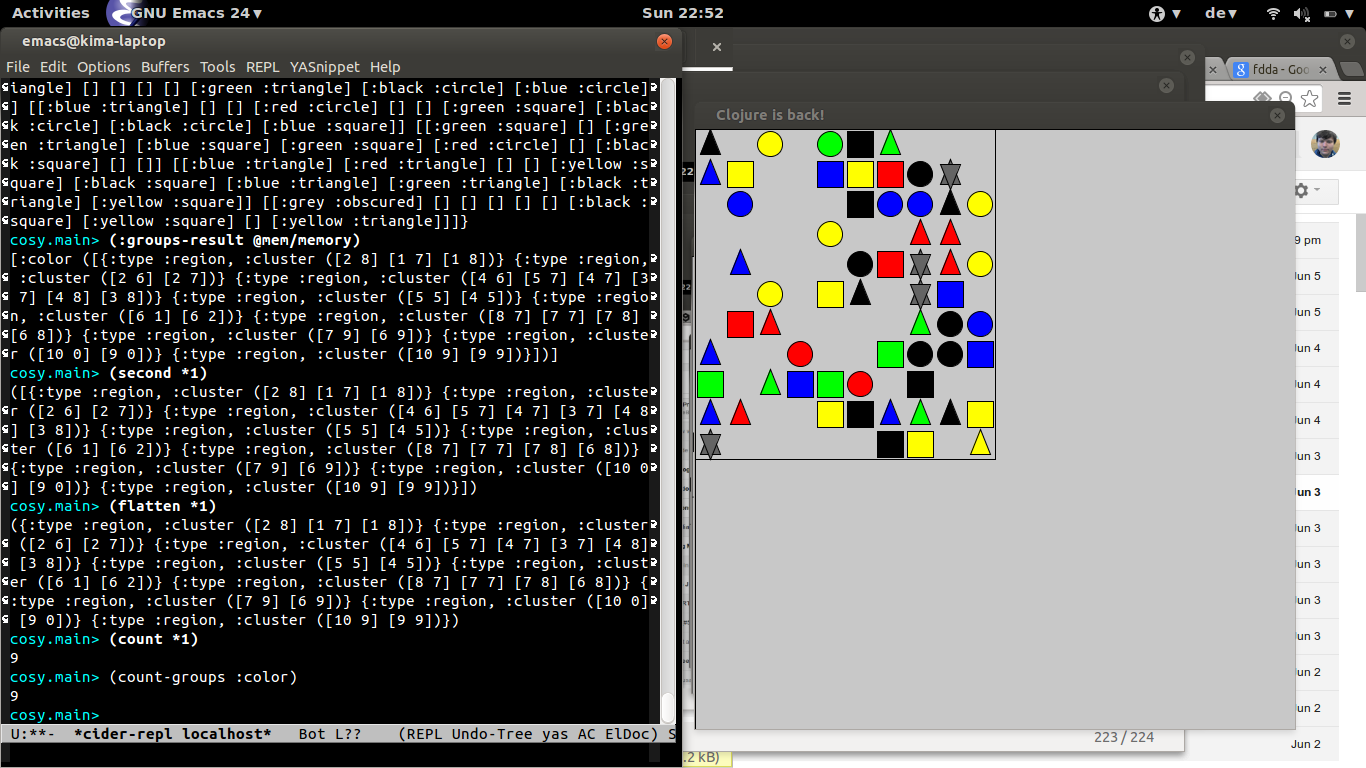
\includegraphics[width= 0.7 \textwidth]{color_groups_example}
    \caption{Recognizing the groups of color}
    \label{fig:aufbau}
\end{figure}

\begin{figure}[h \begin{figure}[hbtp]
    \centering
    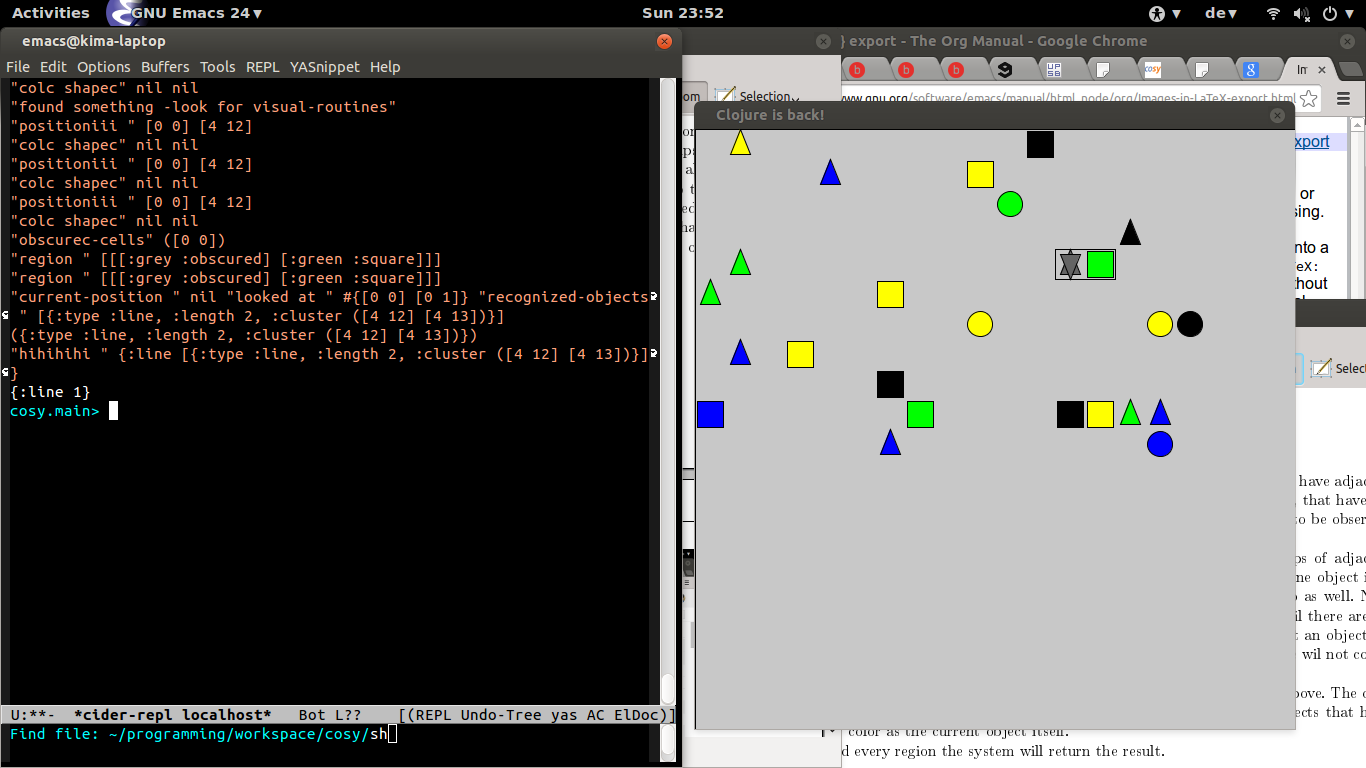
\includegraphics[width= 0.7 \textwidth]{count_obscured}
    \caption{Recognizing one line-like object}
    \label{fig:aufbau}
\end{figure}btp]
    \centering
    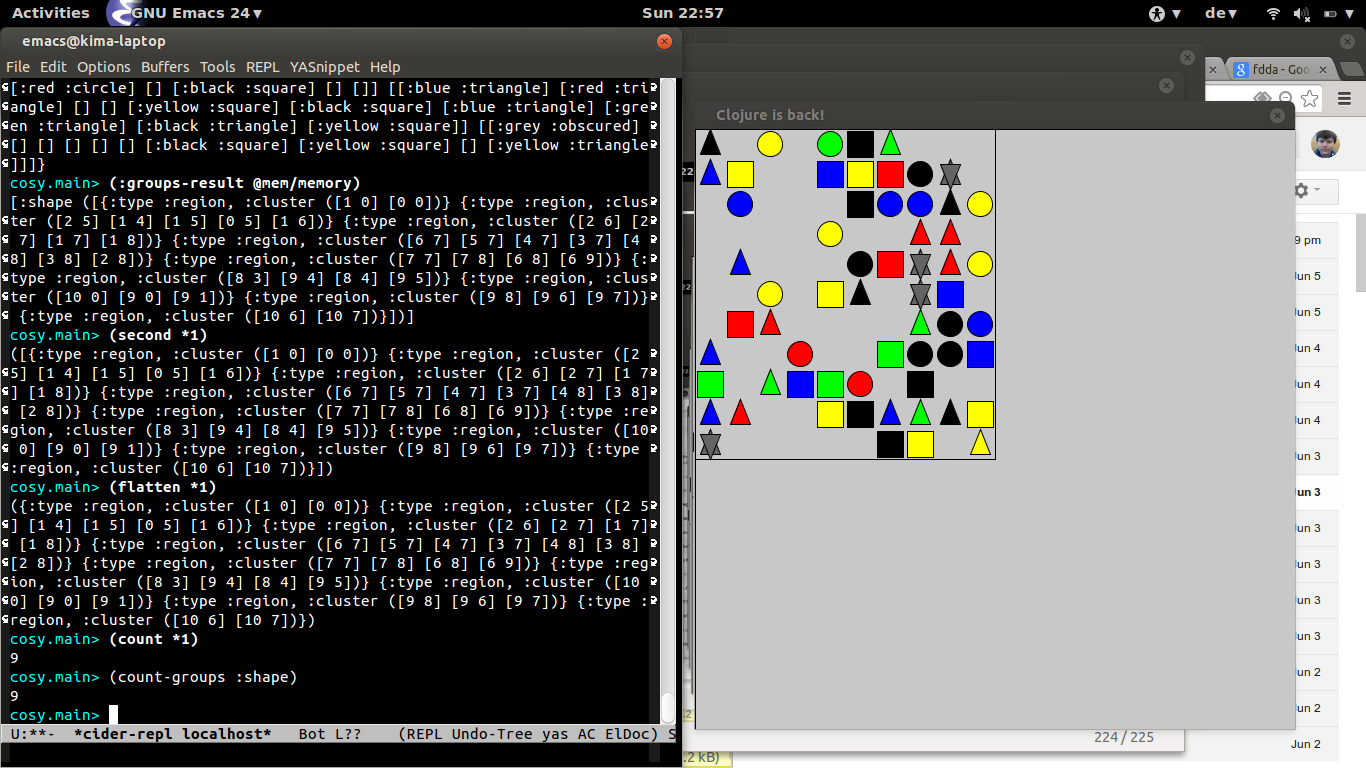
\includegraphics[width= 0.7 \textwidth]{shape_group_example}
    \caption{Recognizing the groups of shape}
    \label{fig:aufbau}
\end{figure}


\section{Excercise2}
\label{sec-2}
We introduced the special object 'obscured' to our cognitive
architecture. A obscured object behaves like a undetermined 
cell in the array. This lets us handle obscured objects uniformely
in the whole cognitive architecture:
\begin{itemize}
\item The regions detected from the peripheral view are increased to 
include the obscured objects because they could obscure a cell
of interest
\item When looking at cells for visual routines we allow obscured cells
as long as we have more known cells than obscured cells.
When we allow obscured cells in that way we have determined some
aspects of them, for example when we recognized a 2x2 square of 
red circles with one obscured object in them we have determined 
for our system that this obscured object is a red circle. This 
means that our system never counts a obscured object as two 
different things
\item because of the uniform handling of obscured objects they are also
supported when counting groups.
\item to count the number of obscured objects we let the peripheral view
filter for regions that contain obscured objects and include all 
directly reachable cells from the obscured objects in them. 
On this region we count all objects/recognize the visual routines
and count how much had obscured objects in them
\end{itemize}


\section{Examples}
\label{sec-3}
1.Here is one example where our System recognizes that there is
one line-like obscured object
 \begin{figure}[hbtp]
      \centering
      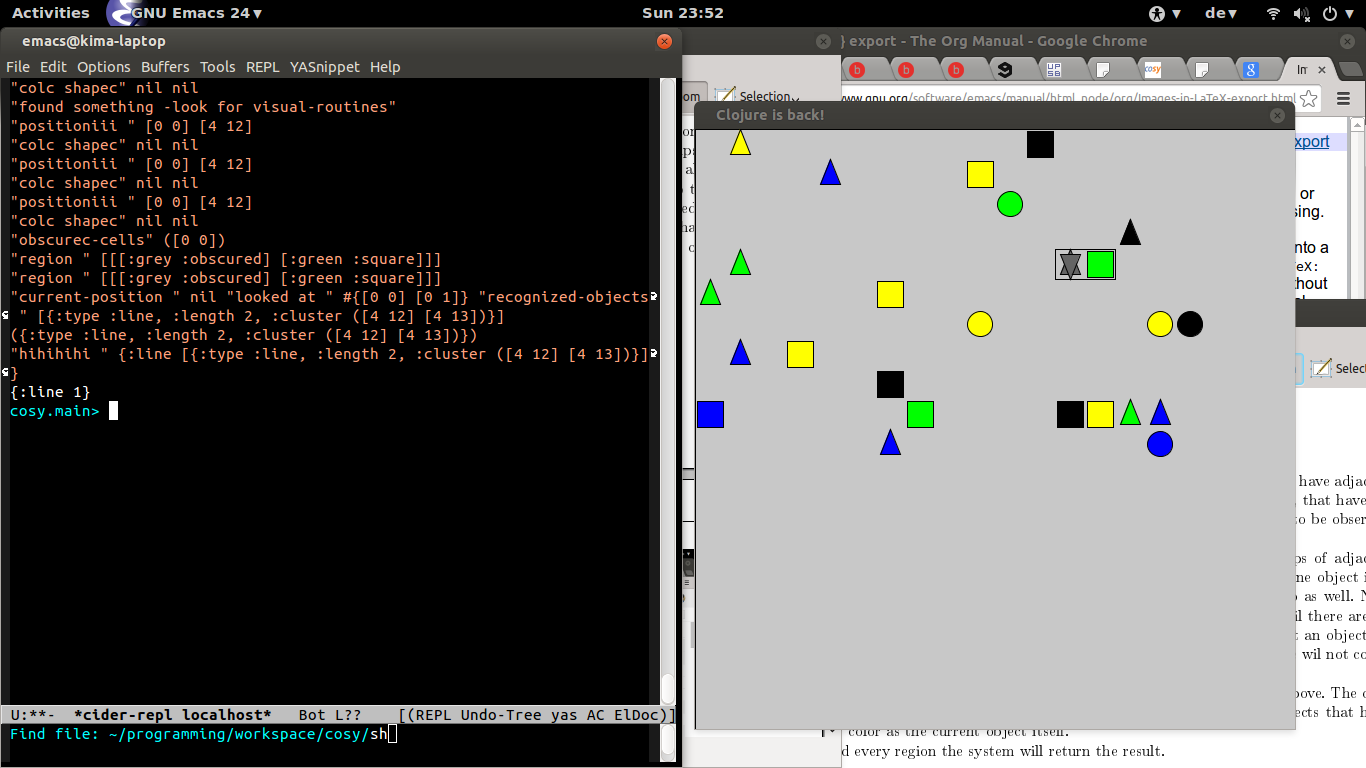
\includegraphics[width= 0.7 \textwidth]{count_obscured}
      \caption{Recognizing one line-like object}
      \label{fig:aufbau}
  \end{figure} \\
2.Another Example of how the system can deal with obscured objects
in all circumstances. Here it has the task to count all red circles
and finds 13. This is the right answer because if recognizes a 
line of two red circles at the bottom of the image with one
being obscured
 \begin{figure}[hbtp]
      \centering
      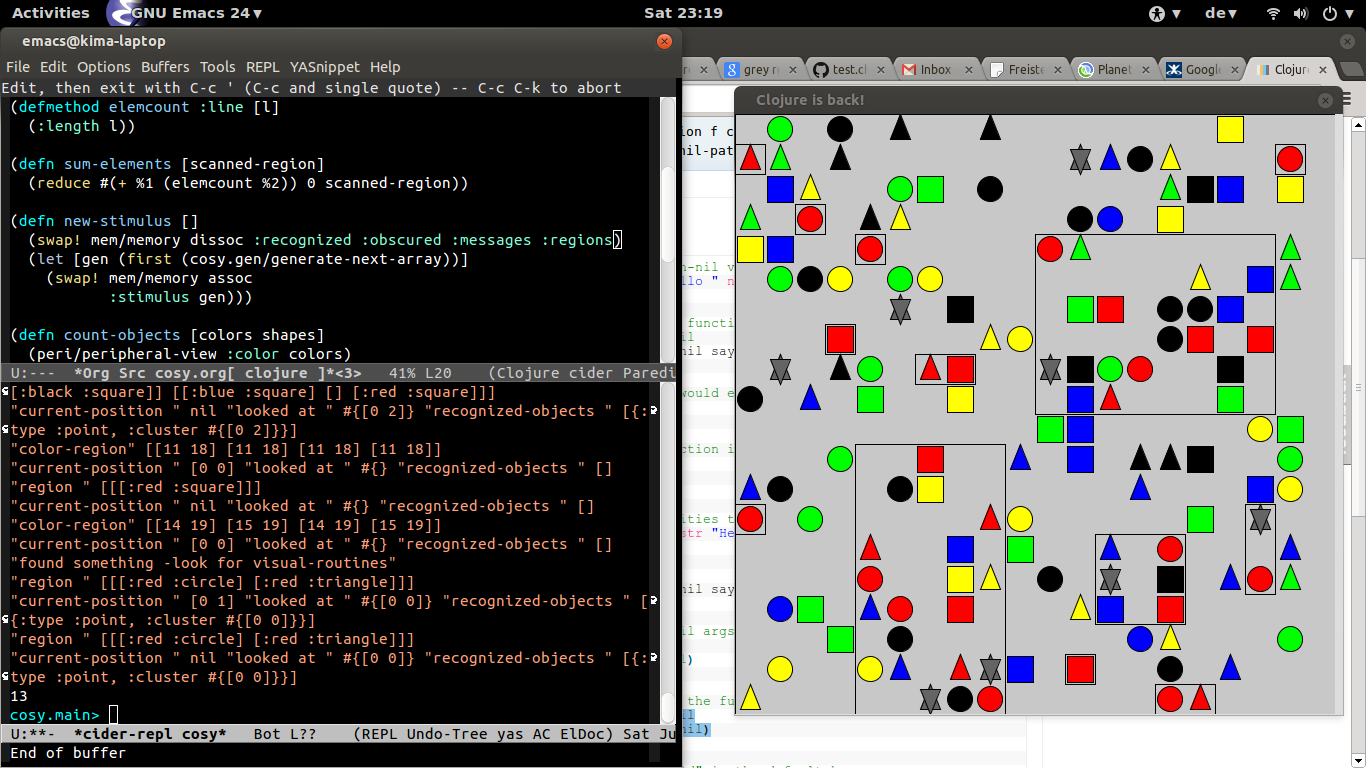
\includegraphics[width= 0.7 \textwidth]{count_red_circles}
      \caption{counting - including obscured objects}
      \label{fig:aufbau}
  \end{figure}
% Emacs 24.3.1 (Org mode 8.2.6)
\end{document}